\documentclass[14pt]{beamer}
\usepackage{./Estilos/BeamerUVM}
\usepackage{./Estilos/ColoresLatex}
\usetheme{Madrid}
\usecolortheme{default}
%\useoutertheme{default}
\setbeamercovered{invisible}
% or whatever (possibly just delete it)
\setbeamertemplate{section in toc}[sections numbered]
\setbeamertemplate{subsection in toc}[subsections numbered]
\setbeamertemplate{subsection in toc}{\leavevmode\leftskip=3.2em\rlap{\hskip-2em\inserttocsectionnumber.\inserttocsubsectionnumber}\inserttocsubsection\par}
% \setbeamercolor{section in toc}{fg=blue}
% \setbeamercolor{subsection in toc}{fg=blue}
% \setbeamercolor{frametitle}{fg=blue}
\setbeamertemplate{caption}[numbered]

\setbeamertemplate{footline}
\beamertemplatenavigationsymbolsempty
\setbeamertemplate{headline}{}


\makeatletter
% \setbeamercolor{section in foot}{bg=gray!30, fg=black!90!orange}
% \setbeamercolor{subsection in foot}{bg=blue!30}
% \setbeamercolor{date in foot}{bg=black}
\setbeamertemplate{footline}
{
  \leavevmode%
  \hbox{%
  \begin{beamercolorbox}[wd=.333333\paperwidth,ht=2.25ex,dp=1ex,center]{section in foot}%
    \usebeamerfont{section in foot} {\insertsection}
  \end{beamercolorbox}%
  \begin{beamercolorbox}[wd=.333333\paperwidth,ht=2.25ex,dp=1ex,center]{subsection in foot}%
    \usebeamerfont{subsection in foot}  \insertsubsection
  \end{beamercolorbox}%
  \begin{beamercolorbox}[wd=.333333\paperwidth,ht=2.25ex,dp=1ex,right]{date in head/foot}%
    \usebeamerfont{date in head/foot} \insertshortdate{} \hspace*{2em}
    \insertframenumber{} / \inserttotalframenumber \hspace*{2ex} 
  \end{beamercolorbox}}%
  \vskip0pt%
}
\makeatother

\makeatletter
\patchcmd{\beamer@sectionintoc}{\vskip1.5em}{\vskip0.8em}{}{}
\makeatother

% \usefonttheme{serif}
\usepackage[clock]{ifsym}
\usetikzlibrary{plotmarks}

\sisetup{per-mode=symbol}
\resetcounteronoverlays{saveenumi}

\title{\Large{Cinemática} \\ \normalsize{Física III}}
\date{}

% Macro para agregar el logo de UVM en cada slide de la presentación

\addtobeamertemplate{frametitle}{}{%
\begin{tikzpicture}[remember picture,overlay]
\coordinate (logo) at ([xshift=-1.5cm,yshift=-0.8cm]current page.north east);
% \fill[devryblue] (logo) circle (.9cm);
% \clip (logo) circle (.75cm);
\node at (logo) {
\includegraphics[width=2.1cm]{Imagenes/logo_UVM.png}};
\end{tikzpicture}}


\begin{document}
\maketitle
  
\section*{Contenido}
\frame{\frametitle{Contenido} \tableofcontents[currentsection, hideallsubsections]}


\section{Cinemática}
\frame{\tableofcontents[currentsection, hideothersubsections]}
\subsection{Conceptos}

\begin{frame}
\frametitle{¿Qué es la mecánica?}
La \textocolor{ao}{mecánica} es la rama de la Física que se encarga del estudio de los cuerpos en movimiento; \pause se divide en \pause \textocolor{burgundy}{cinemática} \pause y \textocolor{darkgreen}{dinámica}.
\end{frame}
\begin{frame}
\frametitle{Cinemática}
La cinemática es la parte de la mecánica que estudia los diferentes tipos de movimiento de los objetos sin atender las causas que lo produjeron.
\end{frame}
\begin{frame}
\frametitle{Movimiento}
Es el cambio de lugar que experimenta un cuerpo dentro de un espacio determinado.
\end{frame}
\begin{frame}
\frametitle{Sistema de referencia}
Sistema de elementos que sirve para fijar la posición de un cuerpo en movimiento.
\end{frame}
\begin{frame}
\frametitle{Posición}
Es el lugar físico en el que se encuentra un cuerpo dentro de un espacio determinado.
\end{frame}
\begin{frame}
\frametitle{Distancia}
La distancia recorrida por un móvil es una \textocolor{magenta}{magnitud escalar}, \pause ya que sólo interesa saber cuál fue la magnitud de la longitud recorrida por el móvil durante la trayectoria seguida, sin importar en qué dirección lo hizo.
\end{frame}
\begin{frame}
\frametitle{Trayectoria}
Es la línea que une las diferentes posiciones que a medida que pasa el tiempo va ocupando un punto en el espacio, \pause de otra forma, es el camino que sigue el objeto dentro de un movimiento.
\end{frame}
\begin{frame}
\frametitle{Trayectoria}
\begin{figure}
    \centering
    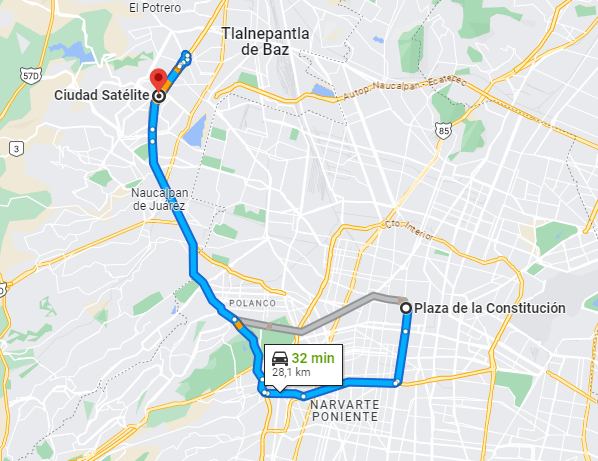
\includegraphics[scale=0.45]{Imagenes/Trayectoria_01.png}
\end{figure}
\end{frame}
\begin{frame}
\frametitle{Tipos de Trayectoria}
Cuando la trayectoria es una línea recta se dice que el movimiento es rectilíneo.
\\
\bigskip
\pause
Cuando la trayectoria es un círculo decimos que el movimiento es circular.
\end{frame}
\begin{frame}
\frametitle{Desplazamiento}
El desplazamiento de un móvil es una \textocolor{cerise}{magnitud vectorial}, ya que corresponde a una distancia medida en una dirección particular entre dos puntos: el de partida y el de llegada.
\end{frame}
\begin{frame}
\frametitle{Desplazamiento}
\begin{figure}
    \centering
    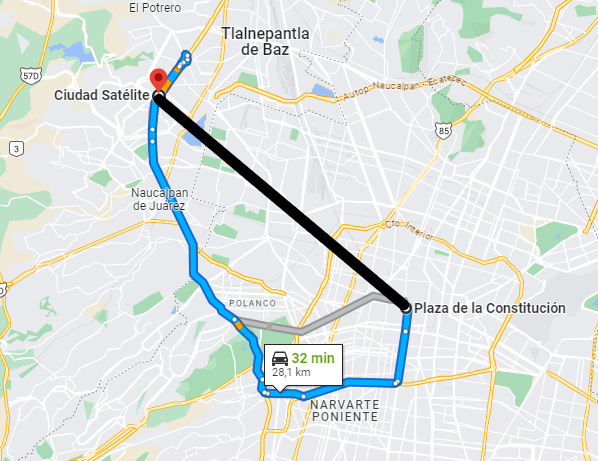
\includegraphics[scale=0.45]{Imagenes/Trayectoria_02.png}
\end{figure}
\end{frame}

\section{Movimiento Rectilíneo Uniforme}
\frame{\tableofcontents[currentsection, hideothersubsections]}
\subsection{Conceptos relevantes}

\begin{frame}
\frametitle{Rapidez}
La \textocolor{auburn}{rapidez} es la distancia recorrida por un objeto en cierto tiempo.
\\
\bigskip
\pause
Es una \textocolor{awesome}{cantidad escalar}, porque se define con una magnitud y una unidad de medida.
\end{frame}
\begin{frame}
\frametitle{Expresión para la rapidez}
La rapidez se obtiene mediante la siguiente expresión:
\pause
\begin{align*}
\text{rapidez} = \dfrac{\text{distancia}}{\text{tiempo}}
\end{align*}
Las unidades son metros por segundo (\unit[per-mode=symbol]{\meter\per\second})
\end{frame}
\begin{frame}
\frametitle{Velocidad}
Es la razón de cambio del desplazamiento de un objeto con respecto al tiempo.
\\
\bigskip
\pause
La velocidad es una \textocolor{byzantine}{magnitud vectorial}.
\end{frame}
\begin{frame}
\frametitle{Expresión para la velocidad}
La velocidad se obtiene mediante la siguiente expresión:
\pause
\begin{eqnarray*}
\begin{aligned}
\text{velocidad} = \dfrac{\text{desplazamiento}}{\text{tiempo}} \pause \hspace*{1.5cm} v = \dfrac{d}{t}
\end{aligned}
\end{eqnarray*}
\pause
Las unidades de la velocidad son metros por segundo (\unit[per-mode=symbol]{\meter\per\second})
\end{frame}
\begin{frame}
\frametitle{Velocidad final}
Es el último instante o momento de la distancia recorrida en el tiempo.
\end{frame}
\begin{frame}
\frametitle{Velocidad media}
Promedio de la suma de todas las distancias y tiempos recorridos.
\end{frame}
\begin{frame}
\frametitle{El triángulo de la velocidad}
En física es común apoyarse con ciertas reglas de tipo visual, que nos ayudarán a simplificar el manejo de una expresión.
\\
\bigskip
\pause
Tal es el caso del \textbf{Triángulo de la velocidad}.
\end{frame}
\begin{frame}
\frametitle{El triángulo de la velocidad}
\begin{figure}
\centering
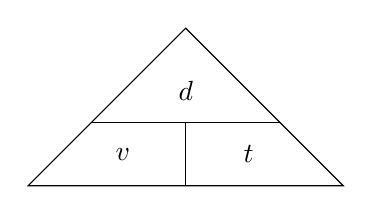
\begin{tikzpicture}
    \draw (0, 0) -- (4, 0) -- (2, 2) -- cycle;
    \draw (2, 0) -- (2, 0.8);
    \draw (0.8, 0.8) -- (3.2, 0.8);

    \node at (2, 1.2) {$d$};
    \node at (1.2, 0.4) {$v$};
    \node at (2.8, 0.4) {$t$};
\end{tikzpicture}
\end{figure}
La idea con esta imagen es recuperar de la expresión, la operación que se necesite si nos piden alguna de las tres variables.
\end{frame}
\begin{frame}
\frametitle{Ejercicio de velocidad}
Un corredor avanza \SI{2}{\kilo\meter} en un tiempo de \SI{15}{\minute}.
\\
\bigskip
\pause
Calcula su velocidad en \unit[per-mode=symbol]{\kilo\meter\per\hour} y en \unit[per-mode=symbol]{\meter\per\second}.
\pause
Revisa que nos piden hacer una conversión de unidades.
\end{frame}
\begin{frame}
\frametitle{Primer paso para la solución al ejercicio}
Se recomienda siempre tener los \textocolor{red}{datos} que nos indica el enunciado.
\pause
\begin{eqnarray*}
\begin{aligned}
\text{desplazamiento} &= \SI{2}{\kilo\meter} \\[0.5em] \pause
\text{tiempo} &= \SI{15}{\minute}
\end{aligned}
\end{eqnarray*}
\end{frame}
\begin{frame}
\frametitle{Segundo paso para la solución al ejercicio}
Nos conviene anotar la \textocolor{cadmiumgreen}{expresión} a utilizar, ya sea de uso directo o tengamos que despejar alguna variable. \pause Nos apoyamos con el triángulo de la velocidad:
\pause
\begin{figure}
\centering
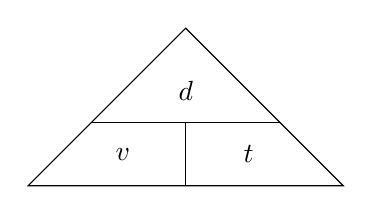
\begin{tikzpicture}
    \draw (0, 0) -- (4, 0) -- (2, 2) -- cycle;
    \draw (2, 0) -- (2, 0.8);
    \draw (0.8, 0.8) -- (3.2, 0.8);

    \node at (2, 1.2) {$d$};
    \node at (1.2, 0.4) {$v$};
    \node at (2.8, 0.4) {$t$};
\end{tikzpicture}
\end{figure}        
\end{frame}
\begin{frame}
\frametitle{Tercer paso para la solución al ejercicio}
Hacemos la sustitución con los valores que nos indica el enunciado:
\pause
\begin{eqnarray*}
\begin{aligned}
v = \dfrac{\SI{2}{\kilo\meter}}{\SI{15}{\minute}} = \pause \SI[per-mode=fraction]{0.1333}{\kilo\meter\per\minute}
\end{aligned}
\end{eqnarray*}
\pause
Nos falta hacer la conversión de unidades.
\end{frame}
\begin{frame}
\frametitle{Haciendo la conversión de unidades}
\begin{eqnarray*}
\begin{aligned}
v &= \SI[per-mode=fraction]{0.1333}{\kilo\meter\per\minute} \left( \dfrac{\SI{60}{\minute}}{\SI{1}{\hour}} \right) = \pause \SI[per-mode=fraction]{8}{\kilo\meter\per\hour} \\[0.5em] \pause
v &= \SI[per-mode=fraction]{0.1333}{\kilo\meter\per\minute} \left( \dfrac{\SI{d3}{\meter}}{\SI{1}{\kilo\meter}} \right) \left( \dfrac{\SI{1}{\hour}}{\SI{3.6d2}{\second}} \right)  = \pause \SI[per-mode=fraction]{2.22}{\meter\per\second}
\end{aligned}
\end{eqnarray*}
\end{frame}
\begin{frame}
\frametitle{Otro ejercicio}
Un ciclista puede alcanzar en una bajada una velocidad de hasta \SI{35}{\kilo\meter\per\hour}.
\\
\bigskip
\pause
¿Qué distancia recorre en una pendiente después de \SI{2}{\minute}?
\end{frame}
\begin{frame}
\frametitle{Datos del enunciado}
\begin{eqnarray*}
\begin{aligned}
v &= \SI{35}{\kilo\meter\per\hour} \\[0.5em] \pause
t &= \SI{2}{\minute} \\[0.5em] \pause
d &= \, ?
\end{aligned}
\end{eqnarray*}
\end{frame}
\begin{frame}
\frametitle{Expresión a utilizar}
\begin{figure}
\centering
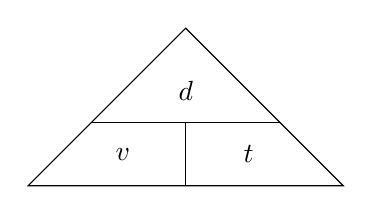
\begin{tikzpicture}
    \draw (0, 0) -- (4, 0) -- (2, 2) -- cycle;
    \draw (2, 0) -- (2, 0.8);
    \draw (0.8, 0.8) -- (3.2, 0.8);

    \node at (2, 1.2) {$d$};
    \node at (1.2, 0.4) {$v$};
    \node at (2.8, 0.4) {$t$};
\end{tikzpicture}
\end{figure}        
\begin{align*}
d = v \, t
\end{align*}
\end{frame}
\begin{frame}
\frametitle{Conversión de unidades}
Antes de hacer la sustitución, debemos de hacer una conversión de unidades para mantener la congruencia con el resultado:
\pause
\begin{eqnarray*}
\begin{aligned}
\SI[per-mode=fraction]{35}{\kilo\meter\per\hour} \left( \dfrac{\SI{d3}{\meter}}{\SI{1}{\kilo\meter}} \right) \left( \dfrac{\SI{1}{\hour}}{\SI{60}{\minute}} \right) = \pause \SI[per-mode=fraction]{583.3}{\meter\per\minute}
\end{aligned}
\end{eqnarray*}
\end{frame}
\begin{frame}
\frametitle{Conversión de unidades}
Ahora sustituimos los valores que ya hemos convertido:
\pause
\begin{eqnarray*}
\begin{aligned}
d &= v \, t \pause = \left( \SI[per-mode=fraction]{583.3}{\meter\per\minute} \right) \left( \SI{2}{\minute} \right) = \\[0.5em] \pause
d &= \SI{1166.6}{\meter}
\end{aligned}
\end{eqnarray*}
\end{frame}
\begin{frame}
\frametitle{Otro ejercicio}
Un auto viaja en una carretera a una velocidad constante de \SI{120}{\kilo\meter\per\hour}
\\
\bigskip
\pause
¿Cuánto tiempo le tomará llegar al poblado más cercano, que está a \SI{180}{\kilo\meter} a esa misma velocidad?
\end{frame}
\begin{frame}
\frametitle{Resolviendo el ejercicio}
\textocolor{red}{Datos:}
\pause
\begin{align*}
v &= \SI{120}{\kilo\meter\per\hour} \\[0.5em]
d &= \SI{180}{\kilo\meter} \\[0.5em]
t &= \, ?
\end{align*}
\end{frame}
\begin{frame}
\frametitle{Resolviendo el ejercicio}
\textocolor{red}{Expresión:}
\pause
\begin{eqnarray*}
\begin{aligned}
v &= \dfrac{d}{t} \\[0.5em] \pause
t &= \dfrac{d}{v}
\end{aligned}
\end{eqnarray*}
\end{frame}
\begin{frame}
\frametitle{Resolviendo el ejercicio}
\textocolor{red}{Sustitución:} Una vez conocida la expresión que debemos de ocupar, procedemos a sustituir los valores que nos indica el enunciado.
\pause
\begin{eqnarray*}
\begin{aligned}
t &= \dfrac{d}{v} \\[0.35em] \pause
t &= \dfrac{\SI{180}{\kilo\meter}}{\SI{120}{\kilo\meter\per\hour}} = \pause \SI{1.5}{\hour}
\end{aligned}
\end{eqnarray*}
\end{frame}
% \begin{frame}
% \frametitle{Ejercicios de Evaluación Continua}
% Con la finalidad de practicar la expresión para la velocidad, desplazamiento y tiempo, se dejarán $6$ ejercicios que contarán como Evaluación Continua, el puntaje a obtener son $6$ puntos.
% \end{frame}
% \begin{frame}
% \frametitle{Ejercicios de Evaluación Continua}
% Los ejercicios estarán en un documento en la asignación en Teams, el plazo de entrega es para el domingo 9 de julio a las 8 pm.
% \end{frame}

\subsection{Intepretando una gráfica}

\begin{frame}
\frametitle{La utilidad de una gráfica}
El movimiento de un cuerpo se puede representar de manera oportuna mediante una gráfica, \pause por lo que será conveniente revisar la manera en la que podemos \enquote{leer} la información contenida en esa gráfica.
\end{frame}
\begin{frame}
\frametitle{El eje horizontal}
Comenzamos reconociendo que en el \textocolor{cadetblue}{eje de las abscisas} tendremos siempre la \textocolor{magenta}{variable temporal}, es decir, el tiempo $t$.
\\
\bigskip
\pause
El tiempo será la \textocolor{alizarin}{variable independiente}.
\end{frame}
\begin{frame}
\frametitle{El eje vertical}
En el \textocolor{ballblue}{eje de las ordenadas}, tendremos la variable de \textocolor{auburn}{desplazamiento}.
\\
\bigskip
\pause
El desplazamiento será la \textocolor{burntumber}{variabe dependiente}.
\end{frame}

\subsection{La recta}

\begin{frame}
\frametitle{Recordando la recta}
Para estudiar el \textocolor{byzantium}{Movimiento Rectilíneo Uniforme}, es necesario recordar la recta y su ecuación.
\end{frame}
\begin{frame}
\frametitle{La gráfica de la recta }
\vspace{-1cm}
\begin{figure}
    \centering
    \begin{tikzpicture}[scale=0.9]
        \draw (0, 0) -- (7.5, 0) node [above, pos=1] {\small{$t \, [\unit{\second}]$}};
        \draw (0, 0) -- (0, 5.3) node [left, pos=1.1] {\small{$d \, [\unit{\meter}]$}};

        \draw (1, 2.3) node {$+$};
        \node at (2, 2.3) {\small{$(x_{i}, y_{i})$}};
        \pause
        \draw [dashed] (1, 0) -- (1, 2.3);
        \node at (1, -0.3) {\small{$x_{i}$}};
        \draw [dashed] (0, 2.3) -- (1, 2.3);
        \node at (-0.6, 2.3) {\small{$y_{i}$}};
        
        \pause
        \draw (4.5, 4.5) node {$+$};
        \node at (5.9, 4.5) {\small{$(x_{f}, y_{f})$}};
        \pause
        \draw [dashed] (4.5, 0) -- (4.5, 4.5);
        \node at (4.5, -0.3) {\small{$x_{f}$}};
        \draw [dashed] (0, 4.5) -- (4.5, 4.5);
        \node at (-0.6, 4.5) {\small{$y_{f}$}};
       
    \end{tikzpicture}
\end{figure}
\end{frame}
\begin{frame}
\frametitle{La gráfica de la recta }
\vspace{-1cm}
\begin{figure}
    \centering
    \begin{tikzpicture}[scale=0.9]
        \draw (0, 0) -- (7.5, 0) node [above, pos=1] {\small{$t \, [\unit{\second}]$}};
        \draw (0, 0) -- (0, 5.3) node [left, pos=1.1] {\small{$d \, [\unit{\meter}]$}};

        \draw (1, 2.45) node {$+$};
        \node at (1, 1.7) {\small{$(x_{i}, y_{i})$}};

        \draw (4.5, 4.32) node {$+$};
        \node at (5.9, 4.5) {\small{$(x_{f}, y_{f})$}};
        
        \draw [thick, color=ao] (0, 2) -- (5, 4.5);

        \pause

        \draw [dashed] (1, 2.45) -- (4.5, 2.45);
        \node at (2.7, 2) {\small{$\Delta x$}};
        \draw [dashed] (4.5, 4.32) -- (4.5, 2.45);
        \node at (4.9, 3.5) {\small{$\Delta y$}};

        \pause

        \node at (6.5, 2.5) {\small{$m = \dfrac{\Delta y}{\Delta x}$}};
    \end{tikzpicture}
\end{figure}
\end{frame}
\begin{frame}
\frametitle{La pendiente de la recta}
La pendiente de la recta es:
\pause
\begin{eqnarray*}
\begin{aligned}
m = \dfrac{\Delta y}{\Delta x} = \pause \dfrac{y_{f} - y_{i}}{x_{f} - x_{i}}
\end{aligned}
\end{eqnarray*}
Para la gráfica de d vs t, la pendiente de la recta es la \textocolor{cobalt}{velocidad} del objeto en movimiento.
\end{frame}
\begin{frame}
\frametitle{La ordenada al origen}
Mientras que la ordenada al origen $b$ representa la posición inicial del objeto antes de que comience el movimiento.
\end{frame}
\begin{frame}
\frametitle{La ordenada al origen}
\vspace{-1cm}
\begin{figure}
    \centering
    \begin{tikzpicture}[scale=0.9]
        \draw (0, 0) -- (7.5, 0) node [above, pos=1] {\small{$t \, [\unit{\second}]$}};
        \draw (0, 0) -- (0, 5.3) node [left, pos=1.1] {\small{$d \, [\unit{\meter}]$}};

        \draw (1, 2.45) node {$+$};
        \node at (1, 1.7) {\small{$(x_{i}, y_{i})$}};
        
        \draw (4.5, 4.32) node {$+$};
        \node at (5.9, 4.5) {\small{$(x_{f}, y_{f})$}};
                
        \draw [thick, color=ao] (0, 2) -- (5, 4.5);

        \node at (-0.4, 2) {\small{$b$}};
    \end{tikzpicture}
\end{figure}
\end{frame}
\begin{frame}
\frametitle{La ecuación de la recta}
La expresión completa para la ecuación de una recta es:
\pause
\begin{align*}
y = m \, x + b
\end{align*}
\end{frame}
\begin{frame}
\frametitle{Caso especial}
\vspace{-1cm}
\begin{figure}
    \centering
    \begin{tikzpicture}[scale=0.9]
        \draw (0, 0) -- (7.5, 0) node [above, pos=1] {\small{$t \, [\unit{\second}]$}};
        \draw (0, 0) -- (0, 5.3) node [left, pos=1.1] {\small{$d \, [\unit{\meter}]$}};

        \foreach [evaluate={\j=int(\x*10)}] \x in {1, 2, 3, 4, 5, 6, 7}
        {    
            \draw (\x, 0.2) -- (\x, -0.2);
            \node at (\x, -0.4) {\small{$\x$}};
        }
        \foreach [evaluate={\j=int(\x*10)}] \x in {1, 2, 3, 4, 5}
        {
            \draw (-0.2, \x) -- (0.2, \x);
            \node at (-0.6, \x) {\small{$\j$}};
        }
        \pause
        \draw [thick, color=ao] (0, 4) -- (7, 4); \pause

        \node at (5, 3) {\small{No hay cambio de posición}}; \pause
        \node at (5, 2.2) {\small{La pendiente de la recta vale $0$}};
        
    \end{tikzpicture}
\end{figure}
\end{frame}
\begin{frame}
\frametitle{Signo de la pendiente}
Debemos de considerar los dos casos con el signo de la pendiente:
\pause
\setbeamercolor{item projected}{bg=bananayellow,fg=ao}
\setbeamertemplate{enumerate items}{%
\usebeamercolor[bg]{item projected}%
\raisebox{1.5pt}{\colorbox{bg}{\color{fg}\footnotesize\insertenumlabel}}%
}
\begin{enumerate}[<+->]
\item La pendiente con \textocolor{cadmiumgreen}{valor positivo}, indica que el objeto \textocolor{cadmiumgreen}{incrementa su velocidad}.
\seti
\end{enumerate}
\end{frame}
\begin{frame}
\frametitle{Signo de la pendiente}
\setbeamercolor{item projected}{bg=bananayellow,fg=ao}
\setbeamertemplate{enumerate items}{%
\usebeamercolor[bg]{item projected}%
\raisebox{1.5pt}{\colorbox{bg}{\color{fg}\footnotesize\insertenumlabel}}%
}
\begin{enumerate}[<+->]
\conti
\item Mientras que una pendiente con \textocolor{carmine}{valor negativo}, nos dice que el objeto \textocolor{carmine}{disminuye su velocidad}.
\end{enumerate}
\end{frame}
\begin{frame}
\frametitle{Pendiente positiva}
\vspace{-1cm}
\begin{figure}
    \centering
    \begin{tikzpicture}[scale=0.9]
        \draw (0, 0) -- (7.5, 0) node [above, pos=1] {\small{$t \, [\unit{\second}]$}};
        \draw (0, 0) -- (0, 5.3) node [left, pos=1.1] {\small{$d \, [\unit{\meter}]$}};

        \draw [thick, color=ao] (0, 2) -- (5, 4.5);
    \end{tikzpicture}
\end{figure}
\end{frame}
\begin{frame}
\frametitle{Pendiente negativa}
\vspace{-1cm}
\begin{figure}
    \centering
    \begin{tikzpicture}[scale=0.9]
        \draw (0, 0) -- (7.5, 0) node [above, pos=1] {\small{$t \, [\unit{\second}]$}};
        \draw (0, 0) -- (0, 5.3) node [left, pos=1.1] {\small{$d \, [\unit{\meter}]$}};

        \draw [thick, color=ao] (1, 4.5) -- (5, 1);
    \end{tikzpicture}
\end{figure}
\end{frame}

\subsection{Estudiando una gráfica}

\begin{frame}
\frametitle{Análisis por intervalos}
El siguiente paso es estudiar una gráfica de desplazamiento contra tiempo, haciéndolo por intervalos de tiempo.
\end{frame}
\begin{frame}
\frametitle{Ejercicio por resolver}
Determina la velocidad del objeto en los intervalos de tiempo:
\pause
\setbeamercolor{item projected}{bg=coquelicot,fg=black}
\setbeamertemplate{enumerate items}{%
\usebeamercolor[bg]{item projected}%
\raisebox{1.5pt}{\colorbox{bg}{\color{fg}\footnotesize\insertenumlabel}}%
}
\begin{enumerate}[<+->]
\item De $0$ a $1$ segundo.
\item De $1$ a $3$ segundos.
\item De $3$ a $4$ segundos.
\item De $4$ a $5$ segundos.
\item De $5$ a $7$ segundos.
\end{enumerate}
\end{frame}
\begin{frame}
\frametitle{La gráfica en estudio}
\vspace{-1cm}
\begin{figure}
    \centering
    \begin{tikzpicture}
        \draw (0, 0) -- (7.5, 0) node [above, pos=1] {\small{$t \, [\unit{\second}]$}};
        \draw (0, 0) -- (0, 5.3) node [left, pos=1.1] {\small{$d \, [\unit{\meter}]$}};

        \foreach [evaluate={\j=int(\x*10)}] \x in {1, 2, 3, 4, 5, 6, 7}
        {    
            \draw (\x, 0.2) -- (\x, -0.2);
            \node at (\x, -0.4) {\small{$\x$}};
        }
        \foreach [evaluate={\j=int(\x*10)}] \x in {1, 2, 3, 4, 5}
        {
            \draw (-0.2, \x) -- (0.2, \x);
            \node at (-0.6, \x) {\small{$\j$}};
        }
        \pause
        \draw [thick, color=ao] (0, 0) -- (1, 1); \pause
        \draw [thick, color=ao] (1, 1) -- (3, 2); \pause
        \draw [thick, color=ao] (3, 2) -- (4, 4); \pause
        \draw [thick, color=ao] (4, 4) -- (5, 5); \pause
        \draw [thick, color=ao] (5, 5) -- (7, 5); \pause
    \end{tikzpicture}
\end{figure}
\end{frame}


\section{Movimiento uniformemente acelerado}
\frame{\tableofcontents[currentsection, hideothersubsections]}
\subsection{La aceleración}

\begin{frame}
\frametitle{Construyendo la aceleración}
Supongamos que un cuerpo se mueve a lo largo de una línea recta y cada segundo se registra que su velocidad aumenta (o disminuye) en \SI{10}{\meter\per\second}.
\end{frame}
\begin{frame}
\frametitle{Construyendo la aceleración}
De manera que al segundo $1$ su velocidad es de \SI{10}{\meter\per\second}, \pause al segundo $2$ es de \SI{20}{\meter\per\second}, \pause al segundo $3$ es \SI{30}{\meter\per\second}, \pause al segundo $4$ es \SI{40}{\meter\per\second}, \pause y por último al segundo $5$, su velocidad es \SI{50}{\meter\per\second}
\end{frame}
\begin{frame}
\frametitle{Preparando una tabla}
\begin{table}
\renewcommand{\arraystretch}{1}
\centering
\begin{tabular}{c | c}
Tiempo [\unit{\second}] & Velocidad [\unit{\meter\per\second}] \\ \hline
$1$ & $10$ \\ \hline
$2$ & $20$ \\ \hline
$3$ & $30$ \\ \hline
$4$ & $40$ \\ \hline
$5$ & $50$ \\ \hline
\end{tabular}
\end{table}
\end{frame}
\begin{frame}
\frametitle{Graficando el cambio de velocidad}
\vspace{-1cm}
\begin{figure}
    \centering
    \begin{tikzpicture}
        \draw (0, 0) -- (6, 0) node [above, pos=1] {\small{$t \, [\unit{\second}]$}};
        \draw (0, 0) -- (0, 5.3) node [left, pos=1.1] {\small{$v \, [\unit{\meter\per\second}]$}};

        \foreach [evaluate={\j=int(\x*10)}] \x in {1, 2, 3, 4, 5}
            {    
            \draw (\x, 0.2) -- (\x, -0.2);
            \node at (\x, -0.4) {\small{$\x$}};

            \draw (-0.2, \x) -- (0.2, \x);
            \node at (-0.6, \x) {\small{$\j$}};
            }

            \foreach \x in {1, 2, 3, 4, 5}
                {
                    \draw [color=blue, fill] (\x, \x) circle (0.4mm);
                    \draw [dashed] (\x, 0) -- (\x, \x);
                    \draw [dashed] (0, \x) -- (\x, \x); \pause
                }
    \end{tikzpicture}
\end{figure}
\end{frame}
\begin{frame}
\frametitle{titulo}
\frametitle{Graficando el cambio de velocidad}
\vspace{-1cm}
\begin{figure}
    \centering
    \begin{tikzpicture}
        \draw (0, 0) -- (6, 0) node [above, pos=1] {\small{$t \, [\unit{\second}]$}};
        \draw (0, 0) -- (0, 5.3) node [left, pos=1.1] {\small{$v \, [\unit{\meter\per\second}]$}};

        \foreach [evaluate={\j=int(\x*10)}] \x in {1, 2, 3, 4, 5}
            {    
            \draw (\x, 0.2) -- (\x, -0.2);
            \node at (\x, -0.4) {\small{$\x$}};

            \draw (-0.2, \x) -- (0.2, \x);
            \node at (-0.6, \x) {\small{$\j$}};
            }

        \foreach \x in {1, 2, 3, 4, 5}
            \draw [color=blue, fill] (\x, \x) circle (0.4mm);

        \draw [thick, red] (1, 1) -- (5, 5);

    \end{tikzpicture}
\end{figure}
\end{frame}
\begin{frame}
\frametitle{Construyendo la aceleración}
Con estos valores reconocemos que la velocidad está variando en \SI{10}{\meter\per\second} cada \SI{1}{\second}, \pause esto es, el cuerpo tiene una aceleración de \SI{10}{\meter\per\square\second}
\end{frame}
\begin{frame}
\frametitle{La aceleración}
Se define la \textocolor{red}{aceleración} \pause como la razón de cambio de la velocidad con respecto al tiempo.
\\
\bigskip
\pause
Es una \textocolor{cerise}{cantidad vectorial}, porque consta de un magnitud o valor, dirección y sentido.
\end{frame}
\begin{frame}
\frametitle{Expresión para la aceleración}
\begin{eqnarray*}
\begin{aligned}
a &= \dfrac{\text{cambio de velocidad}}{\text{intervalo de tiempo}} = \pause \dfrac{\Delta \, v}{\Delta \, t} = \\[1em] \pause
a &= \dfrac{\text{Velocidad final - Velocidad inicial}}{\text{tiempo}} = \\[1em] \pause
a &= \dfrac{v_{f} - v_{i}}{t}
\end{aligned}
\end{eqnarray*}
\end{frame}
\begin{frame}
\frametitle{Consideraciones}
La \textocolor{cobalt}{velocidad inicial} ($v_{i}$) del objeto se define como la velocidad del móvil al inicio del intervalo de tiempo, \pause y que si el objeto se encuentra \textocolor{byzantine}{en reposo}, esta velocidad tiene un valor de cero.
\end{frame}
\begin{frame}
\frametitle{Consideraciones}
La \textocolor{bole}{velocidad final} ($v_{f}$) se define como la velocidad al terminar el intervalo de tiempo.
\end{frame}
\begin{frame}
\frametitle{Signo de la aceleración}
Se considera que un móvil tiene una \textocolor{darkgreen}{aceleración positiva} \pause cuando \textocolor{darkgreen}{aumenta} su velocidad.
\\
\bigskip
\pause
En una gráfica de $v$ vd $t$, la \textocolor{coquelicot}{pendiente de la recta es positiva}.
\end{frame}
\begin{frame}
\frametitle{Signo de la aceleración}
Si \textocolor{blue-violet}{disminuye su velocidad} \pause  tiene \textocolor{blue-violet}{aceleración negativa} (desaceleración o frenado).
\\
\bigskip
\pause
En una gráfica de $v$ vd $t$, la \textocolor{awesome}{pendiente de la recta es negativa}.
\end{frame}
\begin{frame}
\frametitle{Aceleración nula}
De igual modo se considera que un cuerpo no tiene aceleración ($a = 0$) \pause si \textocolor{cerise}{está inmóvil} \pause o si se mueve con \textocolor{bulgarianrose}{velocidad constante}.
\\
\bigskip
\pause
En una gráfica de $v$ vd $t$, la \textocolor{cadetblue!60!black}{pendiente de la recta es cero}.
\end{frame}
\begin{frame}
\frametitle{Enunciado Ejercicio 1}
Un autobús viaja en una carretera a una velocidad de \SI{70}{\kilo\meter\per\hour} y acelera durante \SI{30}{\second} hasta llegar a su límite de velocidad, que son \SI{95}{\kilo\meter\per\hour}.
\\
\bigskip
\pause
¿Cuál fue su aceleración?
\end{frame}
\begin{frame}
\frametitle{Resolviendo el Ejercicio 1}
\textocolor{red}{Datos:}
\pause
\begin{eqnarray*}
\begin{aligned}
v_{i} &= \SI{70}{\kilo\meter\per\hour} \\[0.5em] \pause
v_{f} &= \SI{95}{\kilo\meter\per\hour} \\[0.5em] \pause
t &= \SI{30}{\second} \\[0.5em] \pause
a &= \, ?
\end{aligned}
\end{eqnarray*}
\end{frame}
\begin{frame}
\frametitle{Resolviendo el Ejercicio 1}
\textocolor{red}{Expresión:}
\pause
\begin{align*}
a = \dfrac{v_{f} - v_{i}}{t}
\end{align*}
\end{frame}
\begin{frame}
\frametitle{Conversión de unidades}
Antes de sustituir, ajustamos las unidades de velocidad:
\begin{eqnarray*}
\begin{aligned}
v_{i} &= \left( \SI[per-mode=fraction]{70}{\kilo\meter\per\hour} \right) \pause \left( \dfrac{\SI{1000}{\meter}}{\SI{1}{\kilo\meter}} \right) \pause \left( \dfrac{\SI{1}{\hour}}{\SI{3600}{\second}} \right) = \pause \SI[per-mode=fraction]{19.44}{\meter\per\second} \\[0.5em] \pause
v_{f} &= \SI[per-mode=fraction]{26.38}{\meter\per\second}
\end{aligned}
\end{eqnarray*}
\end{frame}
\begin{frame}
\frametitle{Resolviendo el Ejercicio 1}
\textocolor{red}{Sustitución:}
\pause
\begin{eqnarray*}
\begin{aligned}
a &= \dfrac{\SI[per-mode=fraction]{26.38}{\meter\per\second} - \SI[per-mode=fraction]{19.44}{\meter\per\second}}{\SI{30}{\second}} = \\[0.5em] \pause
a &= \dfrac{\SI[per-mode=fraction]{6.94}{\meter\per\second}}{\SI{30}{\second}} = \\[0.5em] \pause
a &= \SI{0.2313}{\meter\per\square\second}
\end{aligned}
\end{eqnarray*}
\end{frame}
\begin{frame}
\frametitle{Enunciado del Ejercicio 2}
¿Qué tiempo le toma a un auto detenerse si iba a \SI{90}{\kilo\meter\per\hour} antes de aplicar los frenos y desacelerar a \SI{4}{\meter\per\square\second}?
\end{frame}
\begin{frame}
\frametitle{Resolviendo el Ejercicio 2}
\textocolor{red}{Datos:}
\pause
\begin{eqnarray*}
\begin{aligned}
v_{i} &= \SI{90}{\kilo\meter\per\hour} \\[0.5em] \pause
v_{f} &= \SI{0}{\kilo\meter\per\hour} \\[0.5em] \pause
a &= - \SI{4}{\meter\per\square\second} \\[0.5em] \pause
t &= \, ?
\end{aligned}
\end{eqnarray*}
\end{frame}
\begin{frame}
\frametitle{Resolviendo el Ejercicio 2}
\textocolor{red}{Expresión:}
\pause
\begin{eqnarray*}
\begin{aligned}
a &= \dfrac{v_{f} - v_{i}}{t} \\[0.5em] \pause
t &= \pause \dfrac{v_{f} - v_{i}}{a}
\end{aligned}
\end{eqnarray*}
\end{frame}
\begin{frame}
\frametitle{Conversión de unidades}
Antes de sustituir, ajustamos las unidades de velocidad:
\begin{eqnarray*}
\begin{aligned}
v_{i} &= \left( \SI[per-mode=fraction]{90}{\kilo\meter\per\hour} \right) \pause \left( \dfrac{\SI{1000}{\meter}}{\SI{1}{\kilo\meter}} \right) \pause \left( \dfrac{\SI{1}{\hour}}{\SI{3600}{\second}} \right) = \pause \SI[per-mode=fraction]{25}{\meter\per\second}
\end{aligned}
\end{eqnarray*}
\end{frame}
\begin{frame}
\frametitle{Resolviendo el Ejercicio 2}
\textocolor{red}{Sustitución:}
\pause
\begin{eqnarray*}
\begin{aligned}
t &= \pause \dfrac{ \SI{0}{\meter\per\second} - \SI{25}{\meter\per\second}}{- \SI{4}{\meter\per\square\second}} = \\[0.5em] \pause
t &= \dfrac{- \SI{25}{\meter\per\second}}{- \SI{4}{\meter\per\square\second}} = \\[0.5em] \pause
t &= \SI{6.25}{\second}
\end{aligned}
\end{eqnarray*}
\end{frame}


\subsection{Aceleración constante}

\begin{frame}
\frametitle{Tipo de problemas}
Cuando se resuelven problemas donde esté involucrada una \textocolor{red}{aceleración constante}, \pause es importante elegir la fórmula correcta y sustituir los datos conocidos.
\end{frame}
\begin{frame}
\frametitle{Tipo de problemas}
Los problemas se refieren frecuentemente al movimiento de un móvil que \textocolor{ao}{parte del reposo} o que \textocolor{cadmiumgreen}{se detiene} después de cierta velocidad.
\end{frame}
\begin{frame}
\frametitle{Expresiones más utilizadas}
Las siguientes son las fórmulas más utilizadas en el movimiento uniformemente acelerado:
\end{frame}
\begin{frame}
\frametitle{Aceleración y tiempo}
Conociendo la velocidad final $v_{f}$, la velocidad inicial $v_{i}$ y el tiempo $t$, calculamos la aceleración del objeto:
\pause
\begin{align*}
a = \dfrac{v_{f} - v_{i}}{t} \hspace*{1.5cm} \left[ \dfrac{\unit{\meter}}{\unit{\square\second}} \right]
\end{align*}
\end{frame}
\begin{frame}
\frametitle{Aceleración y desplazamiento}
Conociendo la velocidad final $v_{f}$, la velocidad inicial $v_{i}$ y el desplazamiento $d$, calculamos la aceleración del objeto:
\pause
\begin{align*}
a = \dfrac{v_{f}^{2} - v_{i}^{2}}{2 \, d} \hspace*{1.5cm} \left[ \dfrac{\unit{\meter}}{\unit{\square\second}} \right]
\end{align*}
\end{frame}
\begin{frame}
\frametitle{Desplazamiento y tiempo}
Conociendo la velocidad final $v_{f}$, la velocidad inicial $v_{i}$ y el tiempo $t$, calculamos el desplazamiento que recorre el objeto:
\pause
\begin{align*}
d = \left( \dfrac{v_{f} + v_{i}}{2} \right) \, t \hspace*{1.5cm} \left[ \unit{\meter} \right]
\end{align*}
\end{frame}
\begin{frame}
\frametitle{Desplazamiento y aceleración}
Conociendo la la velocidad inicial $v_{i}$, la aceleración $a$ y el tiempo $t$, calculamos el desplazamiento que recorre el objeto:
\pause
\begin{align*}
d = v_{i} \, t + \dfrac{1}{2} \, a \, t^{2} \hspace*{1.5cm} \left[ \unit{\meter} \right]
\end{align*}
\end{frame}
% \begin{frame}
% \frametitle{Enunciado del ejercicio}
% Una tren viaja a una velocidad de \SI{32}{\meter\per\second} y se detiene por completo después de haber recorrido \SI{140}{\meter}
% \\
% \bigskip
% \pause
% ¿Cuál fue su aceleración y en cuánto tiempo se detuvo?
% \end{frame}
% \begin{frame}
% \frametitle{Solución al ejercicio}
% El enunciado nos pide dos cosas:
% \pause
% \setbeamercolor{item projected}{bg=black,fg=white}
% \setbeamertemplate{enumerate items}{%
% \usebeamercolor[bg]{item projected}%
% \raisebox{1.5pt}{\colorbox{bg}{\color{fg}\footnotesize\insertenumlabel}}%
% }
% \begin{enumerate}[<+->]
% \item La aceleración $a$.
% \item El tiempo $t$ que tarda en detenerse.
% \end{enumerate}
% \end{frame}
% \begin{frame}
% \frametitle{Resolviendo el ejercicio}
% \textocolor{red}{Datos:}
% \vspace*{-2cm}
% \begin{align*}
% v_{i} &= \SI{32}{\meter\per\second} \\[0.2em] \pause
% v_{f} &= 0 \\[0.2em]
% d &= \SI{140}{\meter} \\[0.2em]
% a &= \, ? \\[0.2em]
% t &= \, ?
% \end{align*}
% \pause Este ejercicio requiere de dos expresiones.
% \end{frame}
% \begin{frame}
% \frametitle{Resolviendo el ejercicio}
% \textocolor{red}{Expresiones a utilizar}
% \pause
% \begin{eqnarray*}
% \begin{aligned}
% a &= \dfrac{v_{f}^{2} - v_{i}^{2}}{2 \, d} \\[0.5em] \pause
% d &= \left( \dfrac{v_{f} + v_{i}}{2} \right) \, t \pause \hspace{0.2cm} \Rightarrow \hspace*{0.2cm} t = \pause \dfrac{2 \, d}{v_{f} + v_{i}}
% \end{aligned}
% \end{eqnarray*}
% \end{frame}
% \begin{frame}
% \frametitle{Resolviendo el ejercicio}
% \textocolor{red}{Sutitución:}
% \pause
% \begin{eqnarray*}
% \begin{aligned}
% a = \dfrac{ \left( \SI{0}{\meter\per\second} \right)^{2} - \left( \SI{32}{\meter\per\second} \right)^{2} }{2 ( \SI{140}{\meter})} = \pause - \SI{3.66}{\meter\per\square\second}
% \end{aligned}
% \end{eqnarray*}
% El signo negativo nos indica que hay una desaceleración o frenado.
% \end{frame}
% \begin{frame}
% \frametitle{Resolviendo el ejercicio}
% \textocolor{red}{Sustitución:}
% \pause
% \begin{eqnarray*}
% \begin{aligned}
% t = \dfrac{2 (\SI{140}{\meter})}{\SI{32}{\meter\per\second} - \SI{0}{\meter\per\second}} = \pause \SI{8.75}{\second}
% \end{aligned}
% \end{eqnarray*}
% \end{frame}

\section{Caída libre}
\frame[allowframebreaks]{\frametitle{Temas a revisar}  \tableofcontents[currentsection, hideothersubsections]}
\subsection{Definición}

% \begin{frame}
% \frametitle{Planteando el escenario}
% Es bien sabido que, en ausencia de resistencia del aire, \pause todos los objetos que se dejan caer cerca de la superficie de la Tierra caen hacia ella con la misma aceleración constante bajo la influencia de la gravedad de la Tierra.
% \end{frame}
% \begin{frame}
% \frametitle{¿Caída libre?}
% Cuando se usa la expresión objeto en \textocolor{ao}{caída libre} no necesariamente se hace referencia a
% un objeto que se suelta desde el reposo.
% \end{frame}
\begin{frame}
\frametitle{Influencia de la gravedad}
Un objeto en caída libre es cualquier objeto que se mueve libremente sólo bajo la \textocolor{red}{influencia de la gravedad}, \pause sin importar su movimiento inicial.
\end{frame}
% \begin{frame}
% \frametitle{Sentido del lanzamiento}
% Los objetos que se lanzan hacia arriba o abajo y los que se liberan desde el reposo están todos en caída libre una vez que se liberan.
% \end{frame}
% \begin{frame}
% \frametitle{Sentido del lanzamiento}
% Cualquier objeto en caída libre experimenta una aceleración dirigida hacia abajo, sin importar su movimiento inicial.
% \end{frame}
\begin{frame}
\frametitle{Escribiendo la aceleración}
La magnitud de la aceleración de caída libre se denota mediante el símbolo $g$.
% \\
% \bigskip
% \pause
% El valor de $g$ cerca de la superficie de la Tierra disminuye conforme aumenta la altitud.
\end{frame}
\begin{frame}
\frametitle{El valor de la aceleración}
En la superficie de la Tierra, el valor de $g$ es aproximadamente \SI{9.81}{\meter\per\square\second}.
\end{frame}

\subsection{Consideración importante}

\begin{frame}
\frametitle{Resistencia del aire}
% Si se ignora la resistencia del aire \pause y se supone que la aceleración de caída libre no varía con la altitud en distancias verticales cortas, \pause 
El movimiento de un objeto en caída libre que se mueve verticalmente es \textocolor{ao}{equivalente al movimiento de una partícula bajo aceleración constante en una dimensión}.
\end{frame}
% \begin{frame}
% \frametitle{Expresiones para trabajar}
% La \textocolor{carmine}{única modificación} que se necesita hacer en estas ecuaciones para los objetos en caída libre es notar que el movimiento es en la dirección vertical (la dirección $y$) \pause y que la aceleración es hacia abajo y tiene una magnitud de \SI{9.81}{\meter\per\square\second}
% \end{frame}
\begin{frame}
\frametitle{Expresiones para trabajar}
Ocupamos las ecuaciones desarrolladas que vimos para el MUA.
\pause
\begin{minipage}{0.4\linewidth}
\begin{align*}
v_{f} &= v_{i} + g \, t \\[0.5em]
y &= \dfrac{1}{2} \big( v_{i} + v_{f} \big) \, t
\end{align*}
\end{minipage}
\hspace{1cm}
\begin{minipage}{0.4\linewidth}
\begin{align*}
y &= v_{i} \, t + \dfrac{1}{2} g \, t^{2} \\[0.5em]
2 \, g \, y &= v_{f}^{2} - v_{i}^{2} 
\end{align*}
\end{minipage}
\end{frame}
% \begin{frame}
% \frametitle{Sentido de $g$}
% En consecuencia, \pause siempre se elegirá:
% \pause
% \begin{align*}
% a = - g = - \SI{9.81}{\meter\per\square\second}
% \end{align*}
% donde el signo negativo significa que la aceleración de un objeto en caída libre es hacia abajo.
% \end{frame}

\subsection{Ejemplos}
\subsection*{Ejercicio 1}

\begin{frame}
\frametitle{Enunciado del Ejercicio 1}
Se deja caer una moneda de un peso desde la Torre Latinoamericana, parte del reposo y cae libremente.
\\
\bigskip
\pause
Calcula su posición y su velocidad después de $1.0$, $2.0$ y \SI{3.0}{\second}.
\end{frame}
\begin{frame}[plain]
\begin{figure}
\centering
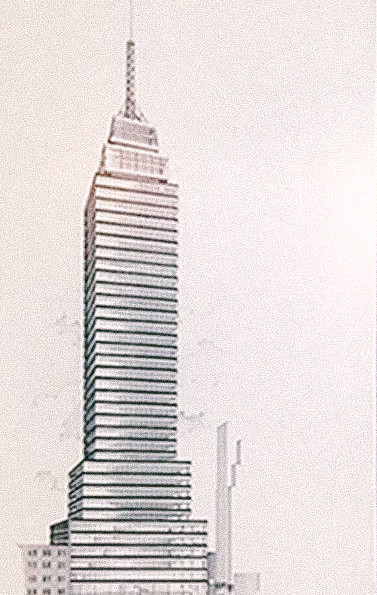
\includegraphics[scale=1.2]{Imagenes/Torre_Latino.jpg}
\end{figure}
\begin{tikzpicture}[overlay]
    \draw (7, 1.3) -- (7, 7) node [left, pos=1] {\small{$y$}};
    \draw (6, 1.3) -- (8, 1.3);
    \draw (6.7, 5.8) -- (7.3, 5.8);
    \draw [fill] (6.4, 5.8) circle (2pt);
\end{tikzpicture}
\end{frame}
\begin{frame}[plain]
\begin{figure}
\centering
\begin{tikzpicture}
    \draw (7, -1) -- (7, 7) node [left, pos=1] {\small{$y$}};

    \node at (2, 4) {\small{$a = -g = - \SI{9.81}{\meter\per\square\second}$}};
    \draw [-stealth, thick] (2.5, 3.5) -- (2.5, 2.5);

    \draw (6, -1) -- (8, -1);
    \draw (6.7, 5.8) -- (7.3, 5.8);
    \draw [fill] (6.4, 5.8) circle (2pt);
    
    \node at (5.4, 5.6) {\small{$v_{0} = 0$}};
    \node at (8.5, 5.6) {\small{$t_{0} = 0 \quad y_{0}=0$}};
    \pause

    \draw (6.7, 4.8) -- (7.3, 4.8);
    \draw [fill] (6.4, 4.8) circle (2pt);
    \node at (5.4, 4.6) {\small{$v_{1} =$ ?}};
    \draw [-stealth, thick] (6.4, 4.8) -- (6.4, 4.3);
    \node at (8.5, 4.6) {\small{$t_{1} = \SI{1}{\second} \quad y_{1}=$?}};
    \pause

    \draw (6.7, 3) -- (7.3, 3);
    \draw [fill] (6.4, 3) circle (2pt);
    \draw [-stealth, thick] (6.4, 3) -- (6.4, 2.3);
    \node at (5.4, 2.8) {\small{$v_{2} =$ ?}};
    \node at (8.5, 2.8) {\small{$t_{2} = \SI{2}{\second} \quad y_{2}=$?}};

    \pause

    \draw (6.7, 1) -- (7.3, 1);
    \draw [fill] (6.4, 1) circle (2pt);
    \draw [-stealth, thick] (6.4, 1) -- (6.4, -0.5);
    \node at (5.4, 0.8) {\small{$v_{3} =$ ?}};
    \node at (8.5, 0.8) {\small{$t_{3} = \SI{3}{\second} \quad y_{3}=$?}};

\end{tikzpicture}        
\end{figure}
\end{frame}
\begin{frame}
\frametitle{Preparando la solución}
Tomaremos el origen $O$ como el punto de partida y la dirección hacia arriba como positiva.
\\
\bigskip
\pause
La coordenada inicial $y_{0}$ y la velocidad inicial $v_{0}$ son ambas cero.
\end{frame}
\begin{frame}
\frametitle{Preparando la solución}
La aceleración es hacia abajo, en la dirección $y$ negativa, \pause así que:
\pause
\begin{align*}
a = - g = - \SI{9.81}{\meter\per\square\second}
\end{align*}
Recordemos que por definición $g$ siempre es positiva.
\end{frame}
\begin{frame}
\frametitle{Preparando la solución}
Por lo que nuestras incógnitas son los valores de $y$ y $v$ en los tres instantes que indica el enunciado.
\end{frame}
\begin{frame}
\frametitle{La expresión a utilizar}
Tenemos las siguientes expresiones:
\pause
\begin{eqnarray*}
\begin{aligned}
y &= v_{0} \, t + \dfrac{1}{2} \, a \, t^{2} \\[0.5em] \pause
v &= v_{0} + a \, t 
\end{aligned}
\end{eqnarray*}
\end{frame}
\begin{frame}
\frametitle{La expresión a utilizar}
En un instante $t$ después de que se suelta la moneda, su posición y velocidad son:
\pause
\begin{eqnarray*}
\begin{aligned}
y &= 0 + \dfrac{1}{2} (-g) \, t^{2} = \pause (\SI{-4.9}{\meter\per\square\second}) \, t^{2} \\[0.5em] \pause
v &= 0 + (-g) \, t = \pause (\SI{-9.8}{\meter\per\square\second}) \, t
\end{aligned}
\end{eqnarray*}
\end{frame}
\begin{frame}
\frametitle{Ocupando los tiempos}
Cuando $t = \SI{1}{\second}$, se tiene que:
\pause
\begin{eqnarray*}
\begin{aligned}
y &= (\SI{-4.9}{\meter\per\square\second}) \, (\SI{1}{\second})^{2} = \pause \SI{-4.9}{\meter} \\[0.5em] \pause
v &= (\SI{-9.8}{\meter\per\square\second}) (\SI{1}{\second}) = \pause \SI{-9.8}{\meter\per\second}
\end{aligned}
\end{eqnarray*}
\end{frame}
\begin{frame}
\frametitle{Los resultados}
Luego de \SI{1}{\second}, la moneda está \SI{4.9}{\meter} debajo del origen ($y$ es negativa), \pause y tiene una velocidad hacia abajo ($v$ es negativa) con magnitud de \SI{9.8}{\meter\per\second}.
\end{frame}
\begin{frame}
\frametitle{Evaluación continua}
La posición y velocidad a los \SI{2.0}{\second} y \SI{3.0}{\second} se obtienen de la misma manera.
\pause
Se puede demostrar que:
\begin{table}
\centering
\begin{tabular}{c | c | c}
Tiempo & Posición $(y)$& Velocidad $(v)$ \\ \hline
\SI{2.0}{\second} & \SI{-19.6}{\meter} & \SI{-19.6}{\meter\per\second} \\ \hline
\SI{3.0}{\second} & \SI{-44.1}{\meter} & \SI{-29.4}{\meter\per\second} \\ \hline
\end{tabular}
\end{table}
\end{frame}
\begin{frame}
\frametitle{Enunciado del Ejercicio 2}
Un niño lanza hacia abajo una piedra con una velocidad de \SI{2}{\meter\per\second} desde lo alto de un árbol de \SI{7}{\meter} de altura. 
\\
\bigskip
\pause
Calcula en cuánto tiempo llegará al piso y con qué velocidad lo hará.
\end{frame}
\begin{frame}
\frametitle{Resolviendo el ejercicio}
\vspace*{-0.3cm}
\textocolor{red}{Datos:}
\pause
\begin{minipage}[t]{0.4\linewidth}
\begin{align*}
v_{i} &= \SI{2}{\meter\per\second} \\[0.5em]
y &= \SI{7}{m} \\[0.5em]
g &= \SI{9.81}{\meter\per\square\second}
\end{align*}
\end{minipage}
\hspace{0.2cm}
\pause
\begin{minipage}[t]{0.4\linewidth}
\begin{align*}
v_{f} = \, ? \\[0.5em]
t = \, ?
\end{align*}
\end{minipage}
\end{frame}
\begin{frame}
\frametitle{¿Qué expresión debemos de usar?}
\vspace*{-1cm}
\begin{minipage}[t]{0.4\linewidth}
\begin{align*}
y &= \dfrac{1}{2} \big( v_{i} + v_{f} \big) \, t  \\[0.5em]
y &= v_{i} \, t + \dfrac{1}{2} g \, t^{2}
\end{align*}
\end{minipage}
\begin{minipage}[t]{0.4\linewidth}
\begin{align*}
v_{f} &= v_{i} + g \, t \\[0.5em]
2 \, g \, y &= v_{f}^{2} - v_{i}^{2} 
\end{align*}
\end{minipage}
\end{frame}
\begin{frame}
\frametitle{Resolviendo el ejercicio}
\textocolor{red}{Expresiones:}
\pause
\begin{eqnarray*}
\begin{aligned}
% y &= \dfrac{v_{f}^{2} - v_{i}^{2}}{2 \, g} \\[0.35em] \pause
2 \, g \, y &= v_{f}^{2} - v_{i}^{2} \\[0.35em] \pause
v_{f}^{2} &= 2 \, g \, y + v_{i}^{2} \\[0.35em] \pause
v_{f} &= \sqrt{2 \, g \, y + v_{i}^{2}} 
\end{aligned}
\end{eqnarray*}
\end{frame}
\begin{frame}
\frametitle{Resolviendo el ejercicio}
\vspace*{-1cm}
\textocolor{red}{Expresiones:}
\begin{eqnarray*}
\begin{aligned}
v_{f} &= v_{i} + g \, t \\[0.5em] \pause
g \, t &= v_{f} - v_{i} \\[0.5em] \pause
t &= \dfrac{v_{f} - v_{i}}{g}
\end{aligned}
\end{eqnarray*}
\end{frame}
\begin{frame}
\frametitle{Resolviendo el ejercicio}
\vspace*{-1.5cm}
\textocolor{red}{Sustitución:}
\pause
\begin{eqnarray*}
\begin{aligned}
v_{f} &= \sqrt{2 \left( \SI[per-mode=fraction]{9.81}{\meter\per\square\second}  \right) \left( \SI{7}{\meter} \right) + \left( \SI[per-mode=fraction]{2}{\meter\per\second} \right)^{2}} = \\[0.4em] \pause
v_{f} &= \sqrt{\SI[per-mode=fraction]{137.34}{\square\meter\per\square\second} + \SI[per-mode=fraction]{4}{\square\meter\per\square\second}} = \pause \sqrt{\SI[per-mode=fraction]{141.34}{\square\meter\per\square\second}} = \\[0.4em] \pause
v_{f} &= \SI[per-mode=fraction]{11.88}{\meter\per\second}
\end{aligned}
\end{eqnarray*}
\end{frame}
\begin{frame}
\frametitle{Resolviendo el ejercicio}
\textocolor{red}{Sustitución:}
\pause
\begin{eqnarray*}
\begin{aligned}
t &= \dfrac{\displaystyle \SI[per-mode=fraction]{11.88}{\meter\per\second} - \SI[per-mode=fraction]{2}{\meter\per\second}}{\displaystyle \SI[per-mode=fraction]{9.81}{\meter\per\square\second}} = \\[0.6em] \pause
t &= \dfrac{\displaystyle \SI[per-mode=fraction]{9.88}{\meter\per\second}}{\displaystyle \SI[per-mode=fraction]{9.81}{\meter\per\square\second}} = \pause \SI{1.007}{\second}
\end{aligned}
\end{eqnarray*}
\end{frame}

\section{Tiro vertical}
\frame{\tableofcontents[currentsection, hideothersubsections]}
\subsection{Definición del problema}

\begin{frame}
\frametitle{¿Qué es el tiro vertical?}
Este movimiento se presenta cuando un objeto \textocolor{ao}{se lanza verticalmente hacia arriba}, \pause y se observa que la magnitud de su \textocolor{armygreen}{velocidad va disminuyendo} \pause hasta anularse al \textocolor{cadetblue!70!black}{alcanzar su altura máxima}.
\end{frame}
\begin{frame}
\frametitle{Tiro vertical}
\begin{figure}
    \centering
    \begin{tikzpicture}
        \draw [->] (0, 0) -- (0, 5) node [left, pos=1] {\small{$y$}};
        \draw (-1, 0) -- (4, 0);
        \node at (1.8, 0.2) {\small{$v_{0} > 0$}};
        \draw [-stealth] (1, 0.1) -- (1, 0.6);
        \draw [fill, color=ao] (1, 0.1) circle (0.1cm); \pause
        \draw [dashed] (1, 0.1) -- (1, 1.1);
        \draw [fill, color=ao] (1, 1.1) circle (0.1cm); \pause
        \draw [dashed] (1, 1.1) -- (1, 2.1);
        \draw [fill, color=ao] (1, 2.1) circle (0.1cm); \pause
        \draw [dashed] (1, 2.1) -- (1, 3.1);
        \draw [fill, color=ao] (1, 3.1) circle (0.1cm); \pause
        \draw [dashed] (1, 3.1) -- (1, 4.1);
        \draw [fill, color=ao] (1, 4.1) circle (0.1cm);
        \draw (-0.1, 4.1) -- (0.1, 4.1);
        \node at (-0.8, 4.1) {\small{$h = y_{\text{máx}}$}};
        \node at (1.8, 4.1) {\small{$v_{0} = 0$}};
    \end{tikzpicture}
\end{figure}
\end{frame}
\begin{frame}
\frametitle{¿Qué es el tiro vertical?}
Inmediatamente inicia su regreso para llegar al mismo punto donde fue lanzado y adquiere la misma magnitud de velocidad con la cual partió.
\end{frame}
\begin{frame}
\frametitle{Tiro vertical}
\begin{figure}
    \centering
    \begin{tikzpicture}
        \draw (0, 0) -- (0, 5)  node [left, pos=1] {\small{$y$}};;
        \draw (-1, 0) -- (4, 0);
        \draw [fill, color=ao] (1, 4.1) circle (0.1cm);
        \draw (-0.1, 4.1) -- (0.1, 4.1);
        \node at (-0.9, 4.1) {\small{$h = y_{\text{máx}}$}};
        \node at (1.8, 4.1) {\small{$v_{0} = 0$}};
        \draw [-stealth] (1, 4.1) -- (1, 3.6);
    \end{tikzpicture}
\end{figure}
\end{frame}
\begin{frame}
\frametitle{¿Qué es el tiro vertical?}
Asimismo, el tiempo empleado en subir es el mismo utilizado en bajar.
\end{frame}

\subsection{Expresiones}

\begin{frame}
\frametitle{Expresiones para el tiro vertical}
\vspace*{-1cm}
En conclusión, el tiro vertical experimenta la misma aceleración que la caída libre de los objetos \pause y, por tanto, emplea las mismas ecuaciones.
\\
\pause
\begin{minipage}{0.4\linewidth}
\begin{align*}
v_{f} &= v_{i} + g \, t \\[0.5em]
y &= \dfrac{1}{2} \big( v_{i} + v_{f} \big) \, t
\end{align*}
\end{minipage}
\hspace{1cm}
\begin{minipage}{0.4\linewidth}
\begin{align*}
y &= v_{i} \, t + \dfrac{1}{2} g \, t^{2} \\[0.5em]
2 \, g \, y &= v_{f}^{2} - v_{i}^{2} 
\end{align*}
\end{minipage}   
\end{frame}
\begin{frame}
\frametitle{Expresión para la altura máxima}
Para calcular la altura máxima que alcanza un objeto lanzado verticalmente hacia arriba usamos la ecuación:
\pause
\begin{align*}
h_{\text{máx}} = - \dfrac{v_{0}^{2}}{2 \, g}
\end{align*}
\end{frame}
\begin{frame}
\frametitle{Expresión para el tiempo de subida}
Para calcular el tiempo que tarda en subir utilizamos la ecuación:
\pause
\begin{align*}
t_{\text{subida}} = - \dfrac{v_{0}}{g}
\end{align*}
\end{frame}
\begin{frame}
\frametitle{Tiempo en el aire}
Como el tiempo que tarda en subir es el mismo para bajar, entonces el tiempo de permanencia en el aire será:
\begin{align*}
t_{\text{aire}} = - \dfrac{2 \, v_{0}}{g}
\end{align*}    
\end{frame}
\begin{frame}
\frametitle{Ejercicio tiro vertical}
Un balón de voleibol que se encuentra al nivel del suelo es lanzado verticalmente hacia arriba con una
velocidad de \SI{29.4}{\meter\per\second}.
\end{frame}
\begin{frame}
\frametitle{Cantidades a responder}
\vspace*{-1cm}
Calcula:
\setbeamercolor{item projected}{bg=britishracinggreen,fg=white}
\setbeamertemplate{enumerate items}{%
\usebeamercolor[bg]{item projected}%
\raisebox{1.5pt}{\colorbox{bg}{\color{fg}\footnotesize\insertenumlabel}}%
}
\begin{enumerate}[<+->]
\item ¿Qué altura habrá subido al primer segundo?
\item ¿Qué magnitud de velocidad llevará al primer segundo?
\item ¿Qué altura máxima alcanzará?
\seti
\end{enumerate}
\end{frame}
\begin{frame}
\frametitle{Cantidades a responder}
\vspace*{-1cm}
\setbeamercolor{item projected}{bg=britishracinggreen,fg=white}
\setbeamertemplate{enumerate items}{%
\usebeamercolor[bg]{item projected}%
\raisebox{1.5pt}{\colorbox{bg}{\color{fg}\footnotesize\insertenumlabel}}%
}
\begin{enumerate}[<+->]
\conti
\item ¿Qué tiempo tardará en subir?
\item ¿Cuánto tiempo durará en el aire?
\end{enumerate}
\end{frame}
\begin{frame}
\frametitle{Solución al ejercicio}
\vspace*{-1cm}
\textocolor{red}{Datos:}
\pause
\begin{minipage}[t]{0.4\linewidth}
\begin{eqnarray*}
\begin{aligned}
v_{0} &= \SI{29.4}{\meter\per\second} \\ 
g &= \SI{9.81}{\meter\per\square\second}
\end{aligned}
\end{eqnarray*}
\end{minipage}
\pause
\hspace{0.2cm}
\begin{minipage}[t]{0.4\linewidth}
\begin{eqnarray*}
\begin{aligned}
h_{1 \, s} &= \, ? \\
v_{1 \, s} &= \, ? \\
h_{\text{máx}} &= \, ? \\
t_{\text{h máx}} &= \, ? \\
t_{\text{vuelo}} &= \, ?
\end{aligned}
\end{eqnarray*}
\end{minipage}
\end{frame}
\begin{frame}
\frametitle{Resolviendo el ejercicio}
\vspace*{-1cm}
¿Qué altura habrá subido al primer segundo?
\\
\textocolor{red}{Expresión:}
\pause
\begin{align*}
h = v_{0} \, t + \dfrac{g \, t^{2}}{2}
\end{align*}
\end{frame}
\begin{frame}
\frametitle{Resolviendo el ejercicio}
\vspace*{-1cm}
\textocolor{red}{Sustitución:}
\pause
\begin{eqnarray*}
\begin{aligned}
h_{1 s} &= \left[ \left( \SI[per-mode=fraction]{29.4}{\meter\per\second} \right) (\SI{1}{\second}) \right] + \dfrac{\displaystyle \left( - \SI[per-mode=fraction]{9.8}{\meter\per\square\second} \right)(\SI{1}{\second})^{2}}{2} = \\[0.5em] \pause
h_{1 s} &= \SI[per-mode=fraction]{29.4}{\meter} - \SI[per-mode=fraction]{4.9}{\meter} =  \\[0.5em] \pause
h_{1 s} &= \SI[per-mode=fraction]{24.5}{\meter}
\end{aligned}
\end{eqnarray*}
\end{frame}
\begin{frame}
\frametitle{Resolviendo el ejercicio}
\vspace*{-1cm}
¿Qué magnitud de velocidad llevará al primer segundo?
\\
\textocolor{red}{Expresión:}
\pause
\begin{align*}
v_{f} = v_{0} + g \, t
\end{align*}
\end{frame}
\begin{frame}
\frametitle{Resolviendo el ejercicio}
\vspace*{-1cm}
\textocolor{red}{Sustitución:}
\pause
\begin{eqnarray*}
\begin{aligned}
v_{1 s} &= \left( \SI[per-mode=fraction]{29.4}{\meter\per\second}\right) + \left[ \displaystyle \left( - \SI[per-mode=fraction]{9.8}{\meter\per\square\second} \right) (\SI{1}{\second}) \right] = \\[0.5em] 
v_{1 s} &= \SI[per-mode=fraction]{29.4}{\meter\per\second} - \SI[per-mode=fraction]{9.8}{\meter\per\second} = \\[0.5em]
v_{1 s} &= \SI[per-mode=fraction]{19.6}{\meter\per\second}
\end{aligned}
\end{eqnarray*}
\end{frame} 
\end{document}